% !TEX program = xelatex
\documentclass[czech,12pt,a4paper]{article}
\usepackage[left=35mm,right=20mm,top=25mm,bottom=25mm]{geometry}
\usepackage[autostyle]{csquotes}
\usepackage[czech]{babel}
\usepackage{titling}
\usepackage{graphicx}
\usepackage{caption}
\usepackage[list=true]{subcaption}
\usepackage{acronym}
\usepackage{setspace}
\usepackage{indentfirst}
\usepackage{listings}
\usepackage{tabularx}
\usepackage{changepage}
\usepackage[hidelinks]{hyperref}
\usepackage{xcolor}
\usepackage{sectsty}
\usepackage{tgtermes}
\usepackage{afterpage}
\usepackage{fontspec}

\setmainfont{Calibri}

\newcommand\blankpage{%
    \null
    \thispagestyle{empty}%
    \addtocounter{page}{-1}%
    \newpage}

\definecolor{blue}{RGB}{32, 91, 157}

\graphicspath{ {./final-report/img} }
\setlength{\parindent}{2em}
\setlength{\parskip}{0.1em}
\linespread{1.5}
\sectionfont{\color{blue}\fontsize{16}{20}\selectfont}
\subsectionfont{\color{blue}\fontsize{14}{20}\selectfont}
\subsubsectionfont{\color{blue}\fontsize{12}{20}\selectfont}

\title{PlantHub}
\author{Filip Sikora, Jakub Vantuch}
\date{}

\begin{document}
\renewcommand*\listfigurename{}
\renewcommand{\figurename}{Obr.}
\renewcommand\refname{}

\afterpage{\blankpage}
\begin{titlepage}
	\vspace*{-1.75cm}
	\noindent
\includegraphics[width=\linewidth]{header.png}
	\begin{center}
		\vspace*{4.5cm}
		{\fontsize{19}{20}\selectfont\textcolor{blue}{MATURITNÍ ZKOUŠKA}}
		\vspace*{7mm} \\
		\textbf{\emph{PRAKTICKÁ ZKOUŠKA Z ODBORNÝCH PŘEDMĚTŮ}}
		\vspace*{5.9cm} \\
		{\fontsize{16}{20}\selectfont\textbf{\textcolor{blue}{Zavlažovací systém PlantHub}}} \\
		\vspace*{6mm}
		{\fontsize{16}{20}\selectfont\textbf{\textcolor{blue}{Téma č. 4}}} \\
		\normalsize
	\end{center}
	\vspace*{\fill}
	\renewcommand{\arraystretch}{0.5}
	\begin{tabularx}{\textwidth}{lX@{\hskip 0.75cm}ll}
		Obor vzdělání: & \multicolumn{2}{l}{\textbf{18 – 20 – M/01 Informační technologie}} \\[10pt]
		& \multicolumn{2}{l}{\textbf{Informační technologie}} \\[10pt]
		Třída: & \textbf{4. IT} & Autor práce: & \textbf{Jakub Vantuch, Filip sikora} \\[10pt]
		Školní rok: & \textbf{2021/22} & Vedoucí učitel práce: & \textbf{Ing. Jiří Sumbal} \\[10pt]
		& & Oponent práce: & \textbf{Ing. Beňová Jiřina} \\[10pt]
		\vspace*{1cm}
	\end{tabularx}
\end{titlepage}

\clearpage

\section*{Prohlášení autora}

\vspace*{\fill}

„Prohlašujeme, že jsme tuto práci vypracovali samostatně a použili jsme literárních pramenů a informací, které citujeme a uvádíme v seznamu použité literatury a dalších zdrojů informací.“ \\
\vspace*{0.5cm} \\
\begin{tabularx}{\textwidth}{l@{\hskip 0.75cm}X@{\hskip 1.5cm}X@{\hskip 0.75cm}l}
	Ve Frýdku-Místku, dne: & \dotfill & \dotfill & podpis \\
	& & & \\
	Ve Frýdku-Místku, dne: & \dotfill & \dotfill & podpis \\
\end{tabularx}

\clearpage

\section*{Zadání práce}

\subsection*{Jakub Vantuch}

\begin{itemize}
	\item Hardwarové řešení - stanovení cílů, volba hardware (řídící jednotka, senzory, akční členy)  
	\item Návrh obvodu a plošného spoje
	\item Fyzická realizace
	\item Naprogramování řídící jednotky
	\item Interaktivní ovládání PlantHubu z webového UI
	\item Odladění, ověření funkčnosti
\end{itemize}

\subsection*{Filip Sikora}

\begin{itemize}
	\item Softwarové řešení - stanovení cílů, volba sw platformy a konkrétního software  
	\item Konfigurace RPi jako webového serveru
	\item Vytvoření databáze
	\item Vytvoření front end
	\item Vytvoření back end
	\item Nastavení bezpečnosti
	\item Interaktivní ovládání PlantHubu z webového UI
	\item Odladění, ověření funkčnosti
\end{itemize}

\clearpage

\section*{Anotace}

PlantHub je zavlažovací systém, s plánovaným a automatickým způsobem zavlažování. Nastavení celého systému je možno upravit přes \ac{WUI}, které navíc nabízí i dashboard a prostředí pro manuální ovládání čerpadla. Jádrem našeho systému je mikropočítač \ac{RPi}, který slouží jako hostovací zařízení pro webový server, databázi, a zároveň jako řídící jednotka celého našeho systému. Systém PlantHub dále získává informace o vlhkosti půdy, teplotě, vlhkosti vzduchu, hladině vody a vykresluje je ve svém \underline{\ac{WUI}}. Ve stejné chvíli naměřená data ukládá do databáze v periodě 4 hodin. Jelikož voda časem v nádrži dojde, systém PlantHub snímá stav hladiny vody v nádrži a včas upozorní, že je třeba ji doplnit.

\section*{Klíčová slova}

\noindent zavlažování; automatizace; statistika; mikropočítač; uživatelské rozhraní

\clearpage

\tableofcontents

\clearpage

\section{Úvod} \label{secUvod}

Naším cílem je návrh, sestavení a naprogramování automatického zavlažovacího systému s názvem PlantHub. Systém se skládá z řídící jednotky (stanice), senzorů, čerpadla, nádrže a \space \underline{\ac{WUI}}. Tato stanice pravidelně snímá data ze senzorů měřících teplotu a vlhkost vzduchu, vlhkost půdy a stav hladiny v nádrži, ze které stanice přečerpává vodu. Naměřená data se živě odesílají a zobrazují ve \underline{\ac{WUI}}, ve stejné chvíli se samostatně, v periodě čtyř hodin ukládají do databáze. Přístup k naměřeným datům a \underline{\ac{WUI}} má pouze uživatel lokální sítě, do které je PlantHub připojen.

\underline{\ac{WUI}} je hostované na naší stanici. Uživatel má možnost zobrazení statistik jak živě naměřených dat, tak dat historických. \underline{\ac{WUI}} také nabízí manuální kontrolu nad čerpadlem, nastavením \underline{\ac{WUI}} a samotné řídící jednotky.

Jednotlivé součásti a moduly stanice jsme vybrali podle finanční dostupnosti a adekvátních technických požadavků na přesnost měření. Obvod jsme v testovací verzi postavili na nepájivém poli a ve finální verzi navrhli a objednali vlastní \ac{PCB}. Pro ochranu naší stanice jsme navrhli kryt, který jsme následně vytiskli na 3D tiskárně.

Hlavní program jsme napsali v programovacím jazyce Go, jehož hlavní využití je vytváření backendů webových aplikací. Tento jazyk se nám zalíbil natolik, že jsme se v něm rozhodli vytvořit jak \ac{API}, databázové funkce, tak i hlavní program. Program je rozdělen na několik sekvencí, z toho hlavní jsou měřící sekvence a sekvence controlleru, která pomocí snímání dat z databáze určuje, zda se jedná o první spuštění PlantHubu. Na základě toho určí, jestli se spustí incializační sekvence nebo sekvence samotného zavlažování.

\begin{itemize}
	\item Kapitoly \underline{\ref{secUvod}}, \underline{\ref{secAcronyms}}, \underline{\ref{secZaver}}, \underline{\ref{secObrazky}}, \underline{\ref{secReference}}, \underline{\ref{secSoftware}}, \underline{\ref{secSeznamPriloh}}, \underline{\ref{secPrilohy}} jsme zpracovali společně. 
	\item Kapitoly \underline{\ref{secHardware}}, \underline{\ref{secPCB}}, \underline{\ref{secRealizace}}, \underline{\ref{secProgram}} zpracoval Jakub Vantuch.
	\item Kapitoly \underline{\ref{secWUI}}, \underline{\ref{secDB}}, \underline{\ref{secWebServer}}, \underline{\ref{secDocker}}, \underline{\ref{secBezpecnost}} zpracoval Filip Sikora.
\end{itemize}


\clearpage

\section{Seznam zkratek a pojmů} \label{secAcronyms}
\begin{acronym}
	\acro{WUI}{webové uživatelské rozhraní} \\
		Vysvětleno v kapitole \underline{\ref{secWUI}}.
	\acro{API}{application programming interface} \\
		Spojení pro přenos dat mezi zařízeními nebo programy, v našem případě, pomocí http protokolu.
	\acro{REST}{representaion programming interface} \\
		Definuje strukturu \underline{\ac{API}} tak, že zobrazuje všechna data a vytváří k nim jednoduchý přístup. Protože, ale nenačítá pouze vybraná data, není tento proces vždy vhodný, jelikož může v mnoha případech zpomalovat celou aplikaci. 
	\acro{GraphQL}{graph query language} \\
		Vysvětleno v kapitole \underline{\ref{secGraphQL}}.
	\acro{PCB}{plošný spoj} \\ 
		Předem připravené pájecí pole, vytvořené tak aby přesně odpovídalo danému obvodu.
	\acro{RPi}{Raspberry Pi} \\ 
		Mikropočítač s podporou IoT. Více v kapitole \underline{\ref{secRPi}}.
	\acro{ADC}{analogově digitální převodník} \\ 
		Vysvětleno v kapitole \underline{\ref{secADC}}.
	\acro{DHT11}{digital humidity temperature v.11} \\ 
		Senzor pro čtení hodnot teploty a vlhkosti vzduchu.
	\acro{HC-SR04}{Ultrasonický senzor vzdálenosti} \\ 
		Vysvětleno v kapitole \underline{\ref{secSonic}}.
	\acro{LED}{light emitting diode} \\ 
		Polovodičová součástka vyzařující světlo.
	\acro{DHCP}{dynamic host configuration protocol} \\ 
		Protokol pro automatické přiřazování IP adres v dané síti.
	\acro{SAR}{successive-approximation} \\ 
		Metoda převodu analogového vstupu na digitální. Více v kapitole \underline{\ref{secADC}}.
	\acro{MSB}{most significant bit} \\ 
		Vysvětleno v kapitole \underline{\ref{secADC}}.
	\acro{LSB}{least significant bit} \\ 
		Vysvětleno v kapitole \underline{\ref{secADC}}.
	\acro{Vref}[$ V_{ref}$]{Referenční napětí} \\ 
		Vysvětleno v kapitole \underline{\ref{secADC}}.
	\acro{Vin}[$ V_{in}$]{Vstupní napětí} \\ 
		Vysvětleno v kapitole \underline{\ref{secADC}}.
	\acro{Vdac}[$ V_{dac}$]{Napětí převedené z digitální do analogové hodnoty} \\ 
		Vysvětleno v kapitole \underline{\ref{secADC}}.
\end{acronym}

\clearpage

\section{Hardware} \label{secHardware}

\subsection{Senzory}

\subsubsection{Senzor teploty a vlhkosti vzduchu DHT11}

Senzor \ac{DHT11} se skládá z jednotky pro měření teploty, jednotky pro měření vlhkosti vzduchu a převodníku.

Teplotu měří senzor termistorem. Termistor je keramický polovodič, který zmenšuje svou rezistivitu, když se okolní teplota zvýší.

Vlhkost měří senzor na základě rezistivity substrátu, umístěného mezi dvěma elektrodami. Tento substrát zachytává vlhkost a vytváří tak vodivé prostředí.

\subsubsection{Senzor vlhkosti půdy}

Jedná se o kapacitní senzor, který se skládá ze dvou vodivých desek a převodníku. Čidlo funguje na způsob kapacitoru avšak jeho kapacita je ovlivněna vlhkostí, která ovlivňuje dielektrikum mezi dvěma deskami.

\subsubsection{Analogově digitální převodník MCP3008} \label{secADC}

\underline{\ac{RPi}} má v rámci general-purpose input/output (GPIO) pinů pouze digitální vstupy, protože je ale senzor vlhkosti půdy analogový, museli jsme použít \ac{ADC}.

Pomocí \underline{\ac{ADC}} v integrovaném obvodu s 10-bitovým rozlišením tedy přemapujeme analogový signál do deseti různých digitálních hodnot, kterým se také říká bitové rozlišení. \underline{\ac{ADC}} měří hodnoty od 0 až po 1023 a následně je pomocí Serial Peripheral Interface (SPI) komunikace posílá do \underline{\ac{RPi}}. \underline{\ac{RPi}} metodou \ac{SAR} definuje adresu v binární formě, srozumitelné pro digitální vstup. V první iteraci převodu se na \underline{\ac{SAR}} registru nastaví první bit na logickou hodnotu 1, stane se z něj \ac{MSB}, ten určuje pozici výstupu srovnávání dané iterace. Je nutné mít správné referenční napětí, to totiž určuje\linebreak nejvyšší možnou binární adresu. Adresa v první iteraci teda bude polovinou nejvyšší možné binární adresy + 1. V další iteraci je první bit \ac{LSB}, to je ten bit, který se v dané iteraci používá pro výstup srovnávání a druhý bit se stává \underline{\ac{MSB}}. Srovnává se hodnota zpětné konverze binární adresy s hodnotou analogového vstupu, pokud je větší, na \underline{\ac{MSB}} se nastaví logická hodnota 1, pokud menší tak logická hodnota 0. Podle počtu bitů \underline{\ac{ADC}} se určují iterace a přesnost převedené hodnoty.

\vspace*{1cm}
\noindent Příklad funkcionality, pro jednoduchost se 4-bitovým \underline{\ac{ADC}}. \\

\noindent\ac{Vref}$ = 16V$ \\
\noindent\ac{Vin}$ = 11V$ \\

1. iterace

\ac{Vdac}$ = \frac{1}{2} \underline{\ac{Vref}}$

\begin{center}
	\begin{tabular}{ |c|c|c|c| } 
		\hline
		(\underline{\ac{MSB}}) & & & \\ 
		\hline
		1 & 0 & 0 & 0 \\ 
		\hline
	\end{tabular}
\end{center}

2. iterace

	$\ac{Vdac} = 8$

	$\underline{\ac{Vin}} > \underline{\ac{Vdac}} => \underline{\ac{LSB}} = 1; \underline{\ac{MSB}} = 1$

\begin{center}
	\begin{tabular}{ |c|c|c|c| } 
		\hline
		(\underline{\ac{LSB}}) & (\underline{\ac{MSB}}) & & \\ 
		\hline
		1 & 1 & 0 & 0 \\ 
		\hline
	\end{tabular}
\end{center}

3. iterace

	$\ac{Vdac} = 12$

	$\underline{\ac{Vin}} < \underline{\ac{Vdac}} => \underline{\ac{LSB}} = 0; \underline{\ac{MSB}} = 1$

\begin{center}
	\begin{tabular}{ |c|c|c|c| } 
		\hline
		& (\underline{\ac{LSB}}) & (\underline{\ac{MSB}}) & \\ 
		\hline
		1 & 0 & 1 & 0 \\ 
		\hline
	\end{tabular}
\end{center}

4. iterace

$\ac{Vdac} = 10$

	$\underline{\ac{Vin}} > \underline{\ac{Vdac}} => \underline{\ac{LSB}} = 1; \underline{\ac{MSB}} = 1$

\begin{center}
	\begin{tabular}{ |c|c|c|c| } 
		\hline
		& & (\underline{\ac{LSB}}) & (\underline{\ac{MSB}}) \\ 
		\hline
		1 & 0 & 1 & 1 \\ 
		\hline
	\end{tabular}
\end{center}

\subsubsection{Ultrasonický senzor HC-SR04} \label{secSonic}

\ac{HC-SR04} vydává zvukové vibrace na vysoké frekvenci, neslyšitelné pro lidské ucho. Poté čeká, až se zvuk odrazí zpět od překážky a vypočítá vzdálenost, na základě času měřeného od vysílání zvukové vlny k zpětnému přijmutí.

\subsubsection{Čerpadlo}

Námi zvolené ponorné mini čerpadlo se skládá z DC motoru, na němž je upevněna centrifuga pro čerpání vody a vlastního pouzdra, z kterého vede otvor pro napojení odtokové hadičky. Čerpadlo je připojeno na zdroj napětí a jeho kostra je uzemněna. Bohužel v procesu testování se nám pokazilo čerpadlo, takže jsme museli vymyslet alternativní cestu, která se nakonec ukázala tou lepší variantou. Koupili jsme nové silnější čerpadlo, připojili k němu samostatný zdroj a přidali relé na jeho spouštění, jako je ukázáno v schématu (Obr. \ref{fig:schema-obvodu-cerpadla}), které jsme vytvořili v nástroji EasyEDA \cite{easyeda}. Zdroj \underline{\ac{RPi}} jsme použili jako signální pin pro spínání relé a vše jsme poskládali do samostatného krytu.

\vspace*{1cm}
\begin{figure}[h]
	\centering
	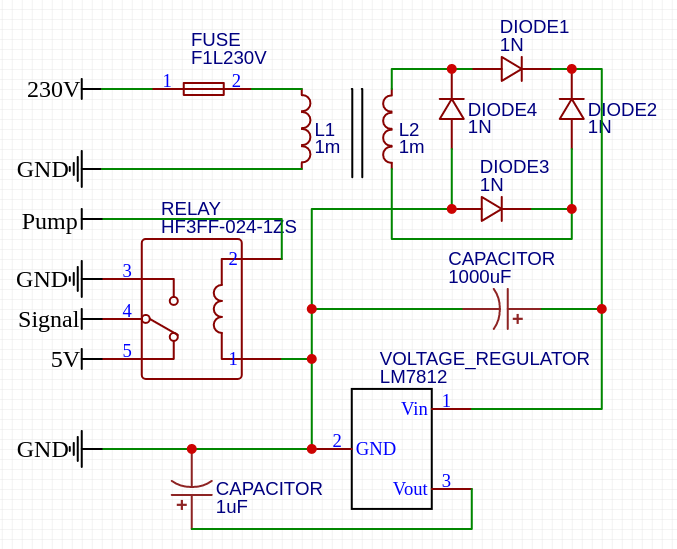
\includegraphics[width=0.67\linewidth]{pump-schema.png}
	\caption{Schéma obvodu čerpadla}
	\label{fig:schema-obvodu-cerpadla}
\end{figure}

\subsubsection{Tranzistor 2N2222}

Protože samotný signální pin neposkytuje dostatečné napětí pro chod čerpadla, ovládáme jej tranzistorem 2N2222. Při výměně čerpadla za jiné, které je spouštěno samostatným relé, jde napětí stále přes tranzistor. Tento tranzistor je bipolární Negative-Positive-Negative tranzistor, to znamená, že jeho polarita je nastavená tak, aby na kolektoru přijímal pozitivní napětí. Díky našemu vyměnitelnému připojení modulů, je možné čerpadlo vyměnit za jiné a přívodný kabel používat jako spouštěč čerpadla jakéhokoliv výkonu a nároků na zdroj. Při používání čerpadla na 5V stačí dva vstupní kontakty + a -, při použití čerpadla se samostatným relé stačí pouze vyměnit kabel za ten se třemi vstupy +, -, a Signal, v tomto případě bude Signal na stejném pinu jako +, pouze přidáme přívodné napětí.

\subsection{Raspberry Pi} \label{secRPi}

Vybrali jsme si jej, protože kombinuje malou velikost a vyšší výpočetní sílu, než Arduino. Musí totiž zvládnout řídit všechny senzory, ukládat data do databáze a zároveň hostuje i samotnou webovou aplikaci.

\subsubsection{Architektura ARM}

Advanced RISC Machines (ARM) je založen na Reduced Instruction Set Computing (RISC) a je to nejnověji používaná CPU architektura. Tyto procesory jsou designované na všechny moderní chytré telefony, zařízení s operačním systémem Android i Apple produkty.

\subsection{Router}

Připojení \underline{\ac{RPi}} do lokální sítě je provedeno pomocí ethernet kabelu do patřičného routeru s \ac{DHCP} mechanismem. Klientský počítač připojený do stejné sítě, si poté může jednoduše zobrazit \underline{\ac{WUI}} hostované na samotném \underline{\ac{RPi}}

\clearpage

\section{Návrh obvodu a plošného spoje} \label{secPCB}

\subsection{Testovací verze}

V prvním kroku jsme si vytvořili grafické znázornění celého obvodu (Obr. \ref{fig:graficke-znazorneni-obvodu}) v nástroji figma \cite{figma}, Testovací verzi našeho obvodu jsme postavili na nepájivém kontaktním poli. Jakmile jsme měli vše plně odzkoušeno a plně otestováno, přešli jsme na profesionálnější řešení.

\noindent\begin{figure}[h]
	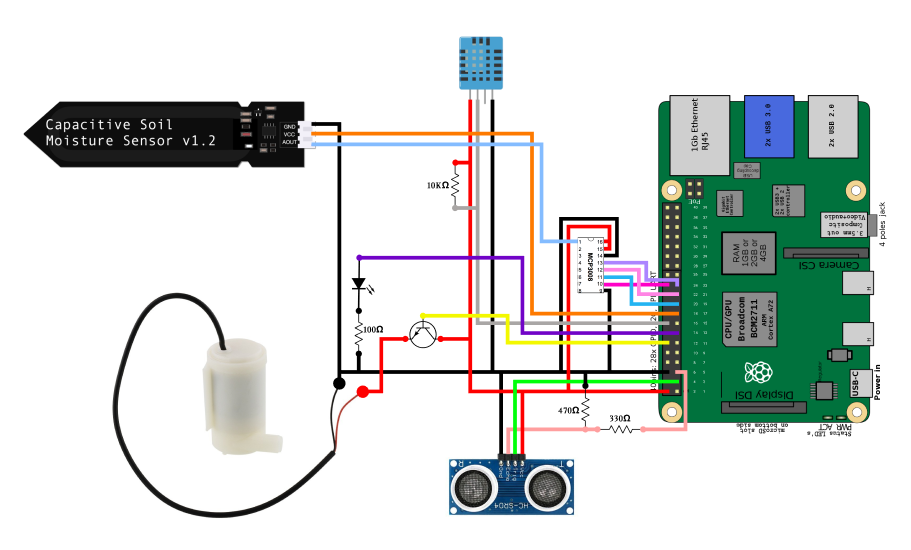
\includegraphics[width=\linewidth]{obvod.png}
	\caption{Grafické znázornění obvodu}
	\label{fig:graficke-znazorneni-obvodu}
\end{figure}

\clearpage

\subsection{Finální verze}

Ve finální verzi jsme navrhli naše vlastní schéma hlavního obvodu (Obr. \ref{fig:schema-obvodu}). Toto schéma jsme si nechali vytisknout společností JLCPCB a po doručení jsme na něj napájeli patřičné komponenty (Obr. \ref{fig:finalni-verze}).

\vspace*{2cm}
\begin{figure}[h]
	\begin{minipage}[t]{0.5\linewidth}
		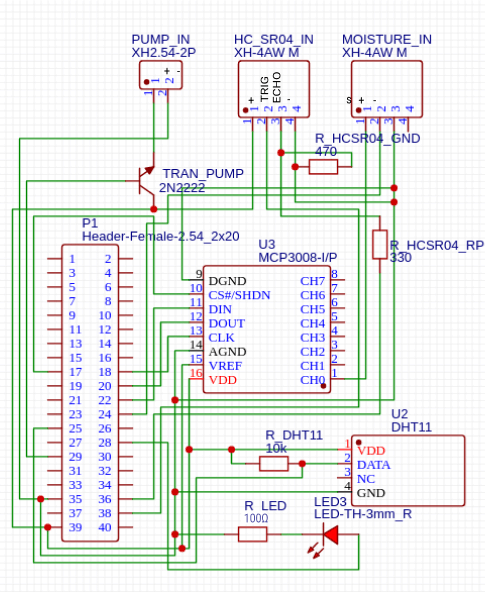
\includegraphics[width=\linewidth]{pcb-schema.png}
		\caption{Schéma obvodu}
		\label{fig:schema-obvodu}
	\end{minipage}
	\hfill
	\begin{minipage}[t]{0.5\linewidth}
		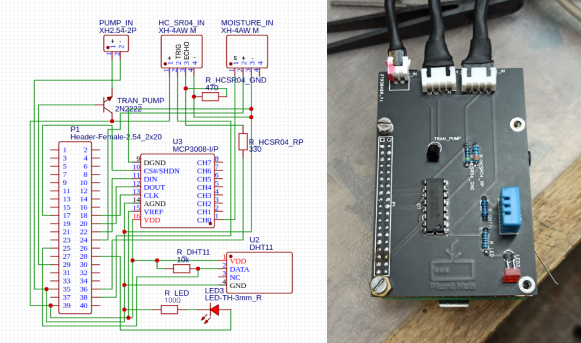
\includegraphics[width=\linewidth]{pcb.png}
		\caption{Finální verze \underline{\ac{PCB}} se senzory}
		\label{fig:finalni-verze}
	\end{minipage}
\end{figure}

\clearpage

\section{Fyzická realizace} \label{secRealizace}

% Vymstila se nám však nepřesnost rozměrů krytu a při vkládání stanice do krytu se nám podařilo zlomit SD kartu s operačním systémem, daty a nasazenými programy. Po reinstalaci operačního systému jsme opravili rozměry vytvořeného modelu krytu a vytiskli kryt podruhé, tentokrát ve správných rozměrech.

\subsection{Pouzdro}

Navrhli jsme vhodné pouzdro (Obr. \ref{fig:pouzdro}) pro naše \underline{\ac{RPi}}, abychom ochránili citlivé elektronické součástky a zároveň měli možnost jednoduše vyjmout stanici z krytu. Pouzdro jsme vytiskli na školní 3D tiskárně pevným Polyethylene terephthalate glycol (PETG) filamentem.

Při první iteraci našeho pouzdra jsme nepřidali dostatečnou toleranci pro SD kartu, která přesahuje hranice PCB o několik milimetrů. Omámeni nadšením z první hmatatelné verze našeho pouzdra, jsme se neopatrně a rychle pokusili, napasovat pouzdro na Raspberry Pi. Naší neopatrností se nám podařilo zmiňovanou SD kartu zlomit. Za odměnu jsme si tedy znova procvičili instalaci a konfiguraci operačního systému Raspberry Pi.

\vspace*{1cm}
\begin{figure}[h]
	\centering
	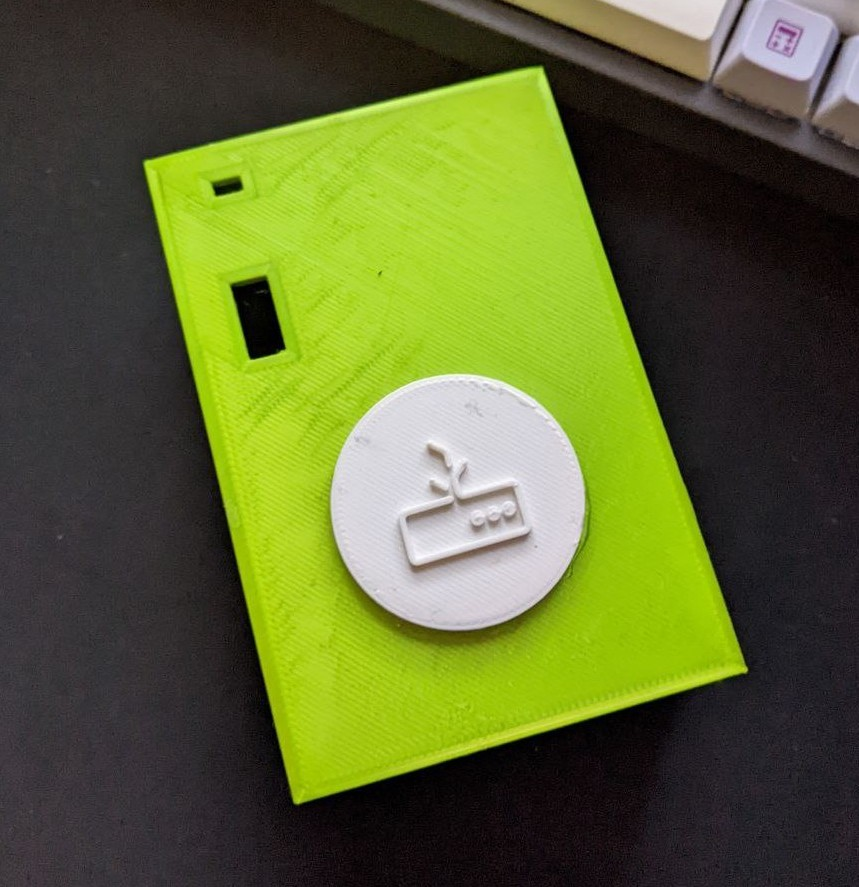
\includegraphics[width=0.67\linewidth]{pouzdro.jpeg}
	\caption{Pouzdro}
	\label{fig:pouzdro}
\end{figure}

\subsection{Hub}

Zkompletovaný hub se tedy skládá z pouzdra, \underline{\ac{RPi}}, \underline{\ac{PCB}} a připojených senzorů, ethernet kabelu a zdrojového kabelu. Jednoduchým způsobem je možno hub rozebrat pro případnou opravu.

\vspace*{1cm}
\begin{figure}[h]
	\centering
	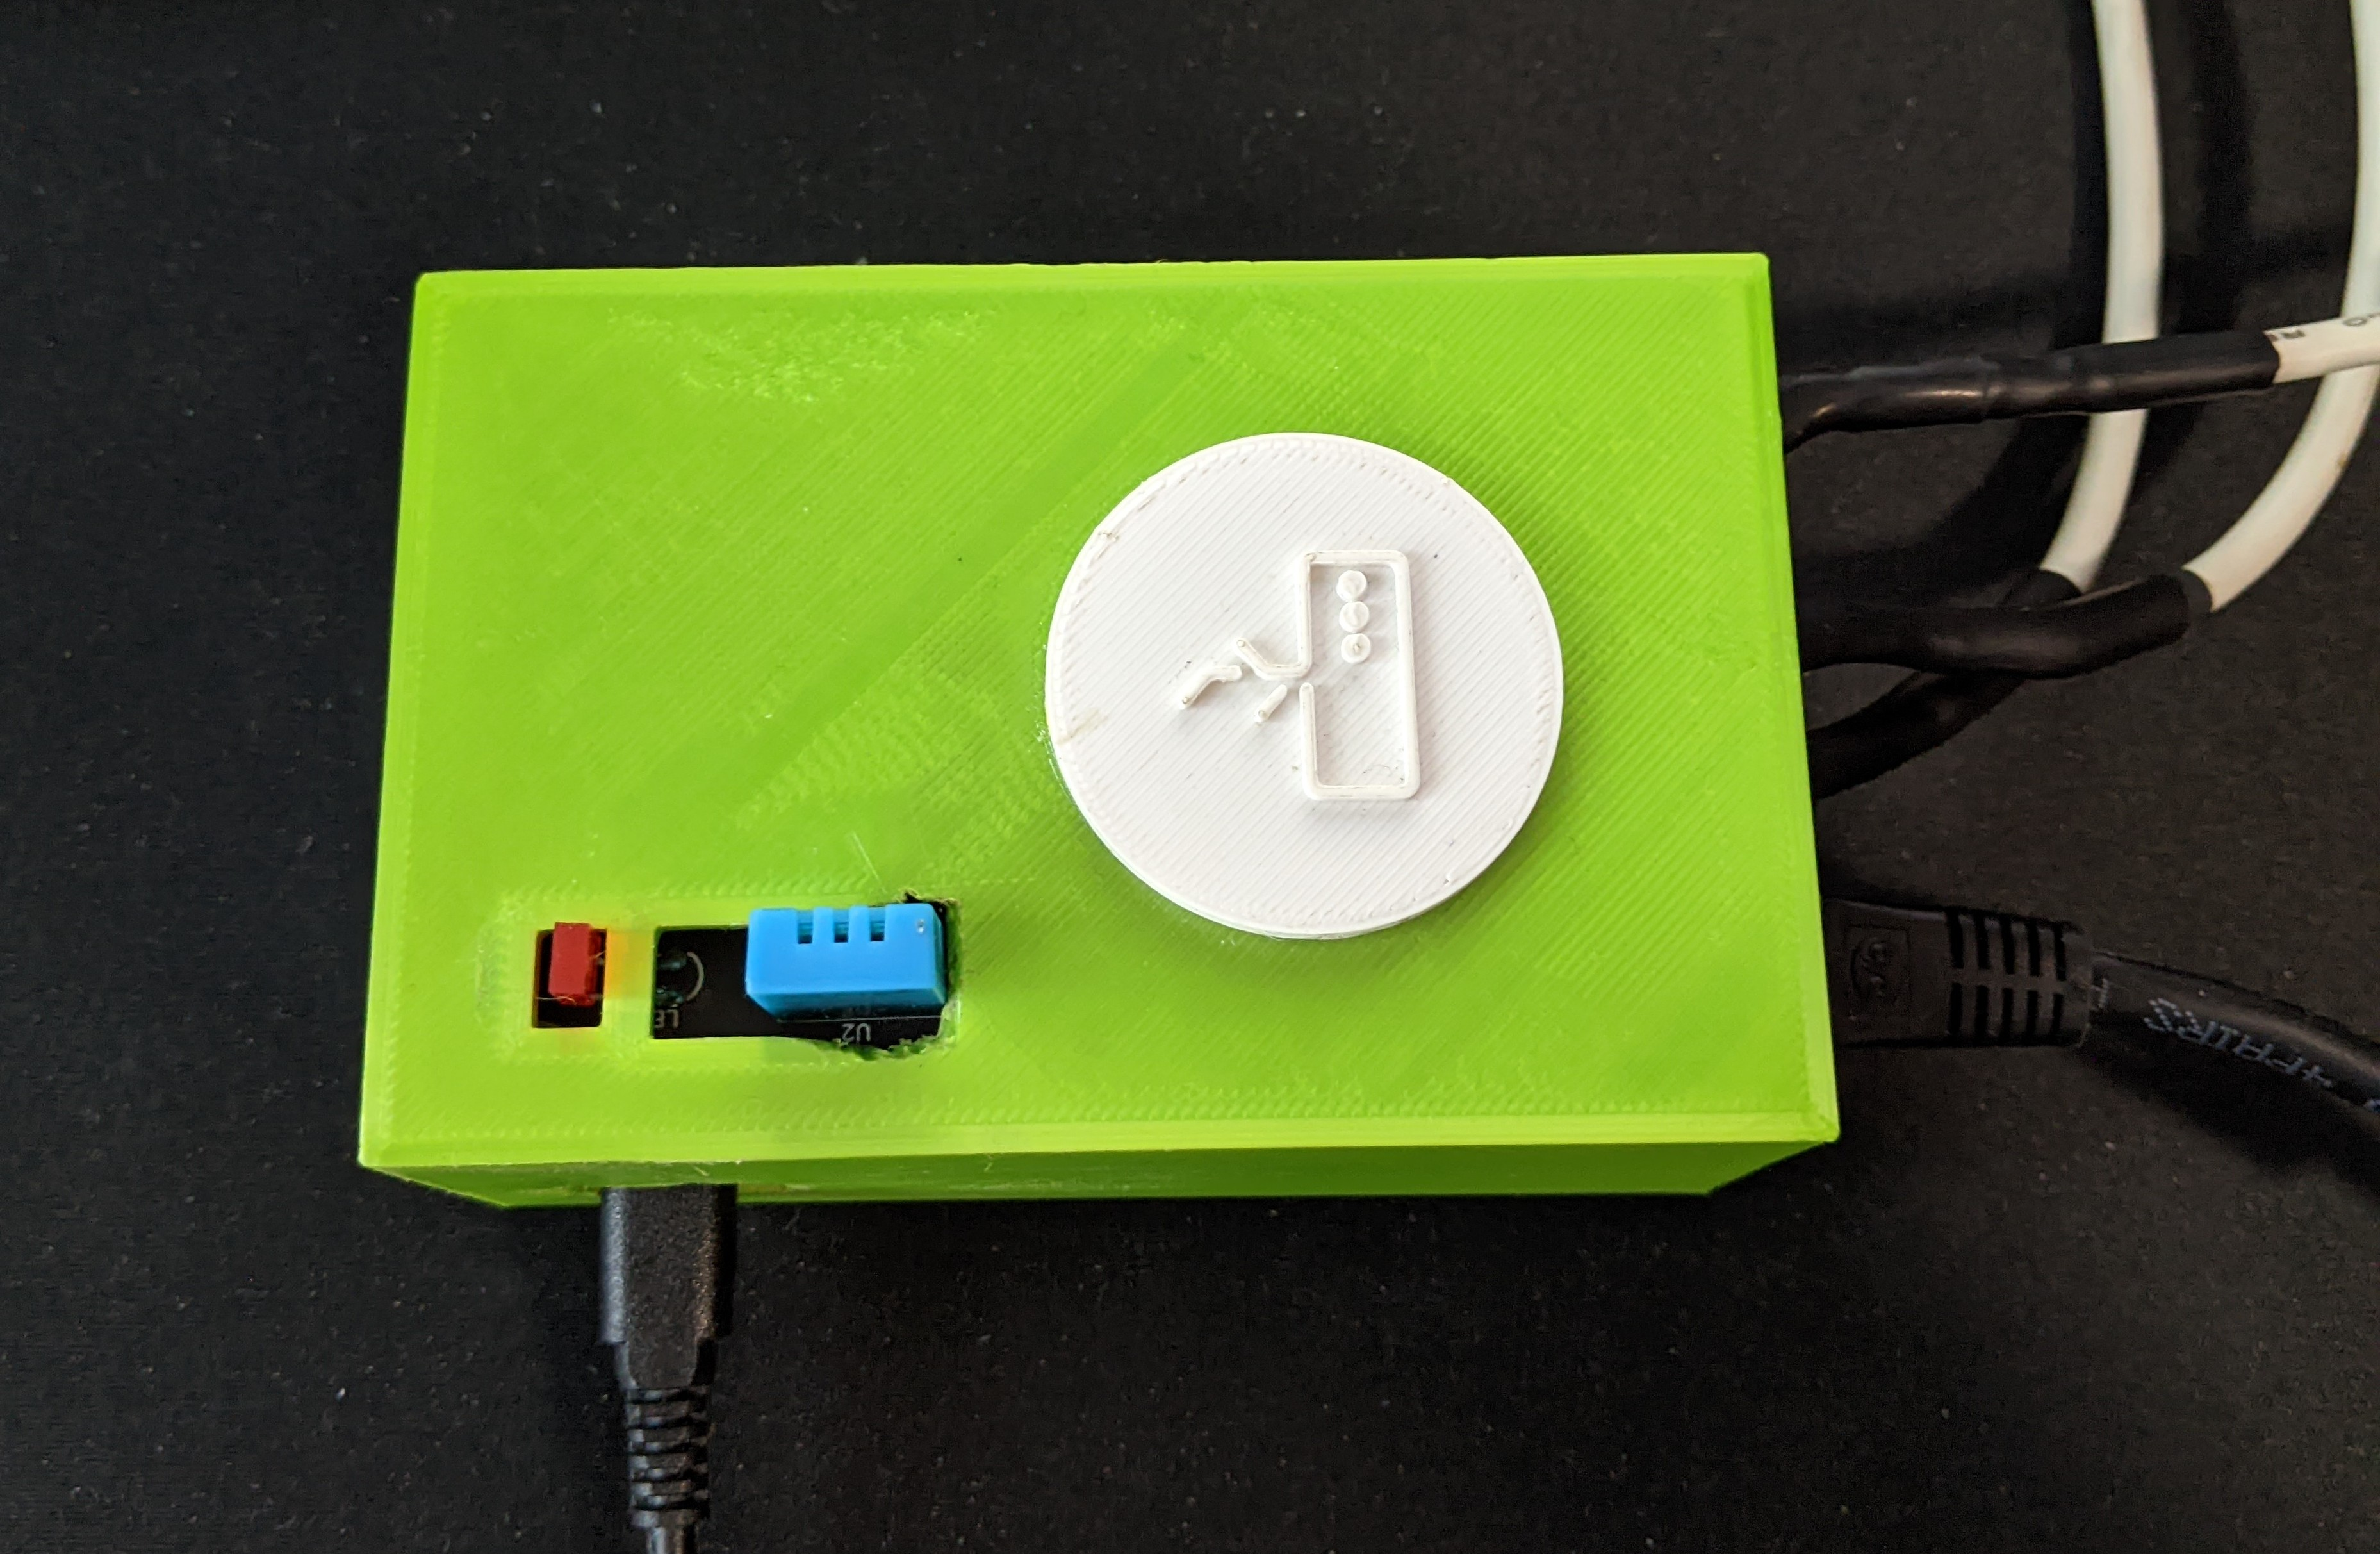
\includegraphics[width=0.82\linewidth]{hub.jpeg}
	\caption{Hub}
\end{figure}

\clearpage

\subsection{Nádrž}

K zavlažování bylo potřeba postavit nádrž na vodu, ze které bude naše čerpadlo přečerpávat vodu k zavlažování. Nejvhodnějším řešením je nádoba s co\linebreak největším objemem, která bude jednoduše přenosná, odolná a nebude složité\linebreak připevnit na ní senzory. Nakonec jsme ji postavili z upraveného 5L pivního soudku, natřeli antikorozní barvou a upravili podle našich potřeb.

\vspace*{1cm}
\begin{figure}[h]
	\centering
	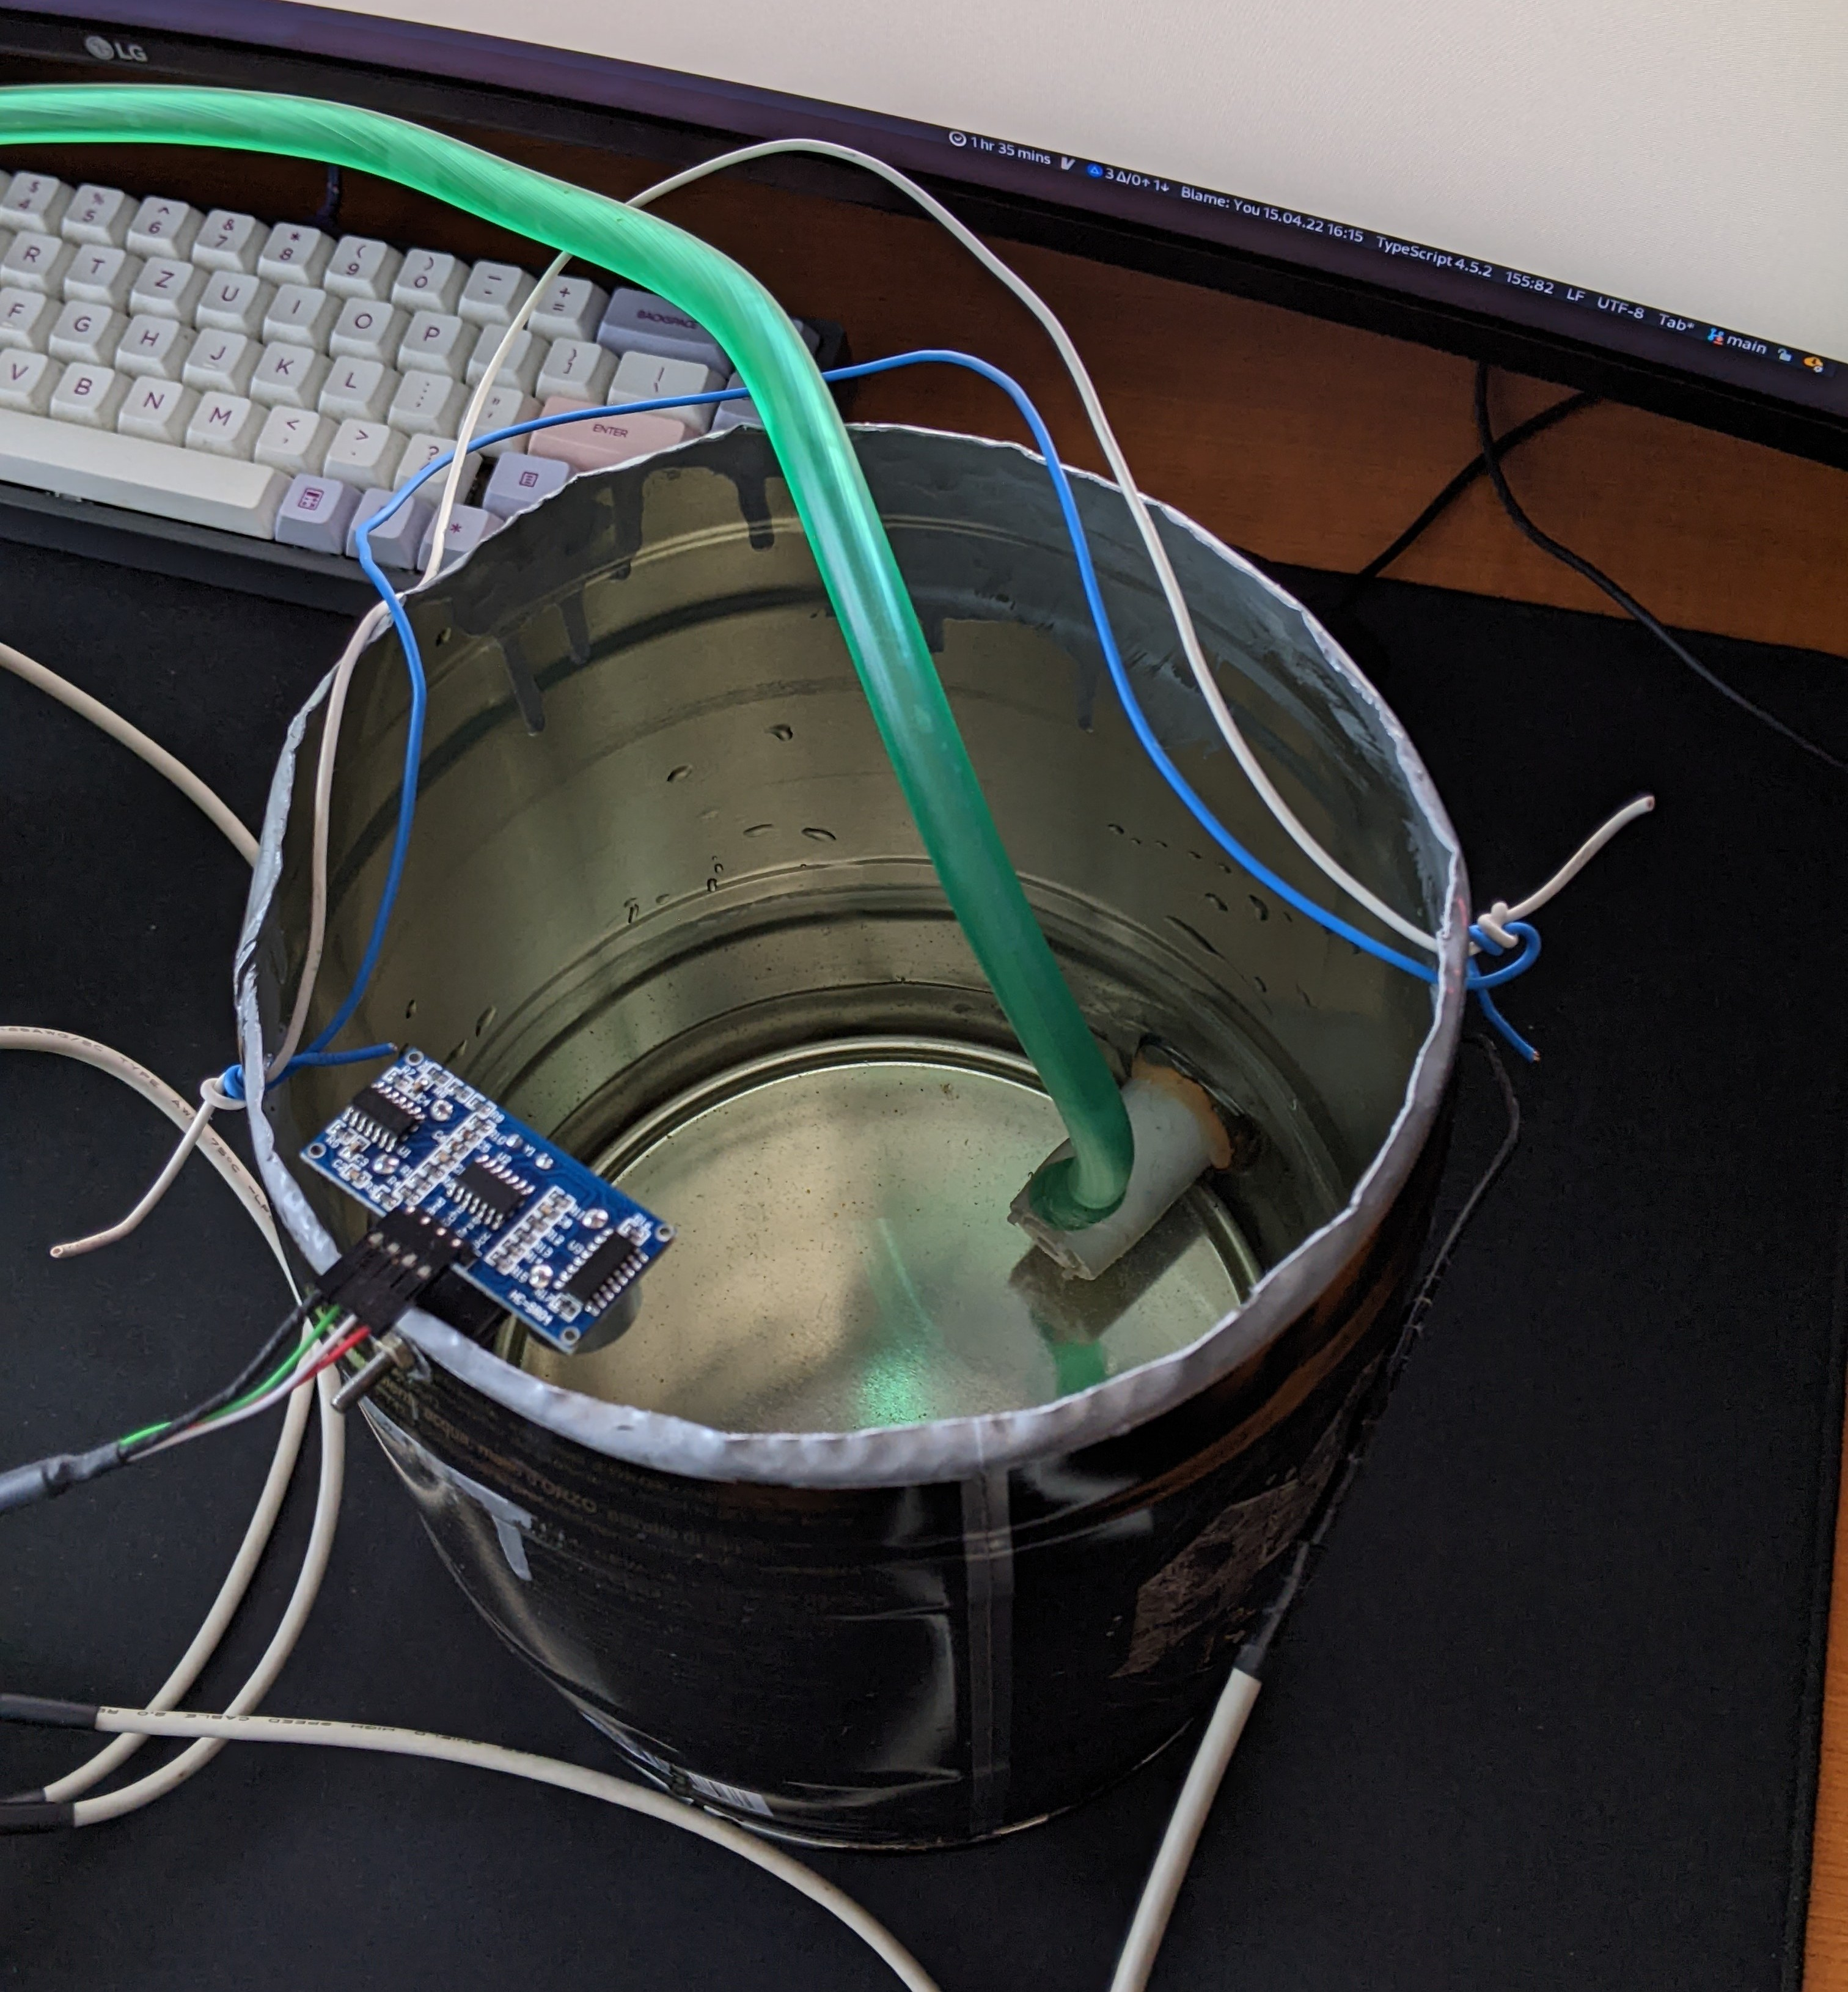
\includegraphics[width=0.7\linewidth]{nadrz.jpeg}
	\caption{Nádrž}
\end{figure}

\clearpage

\subsection{Celý systém}

Celý systém se tedy skládá z Hubu, nádrže, rostliny, routeru a klientského zařízení. Sestavení trvá asi 5 minut, protože musíme počkat, než se načte OS \underline{\ac{RPi}} a následně zapojit všechny modulární části našeho systému.

\begin{figure}[h]
	\centering
	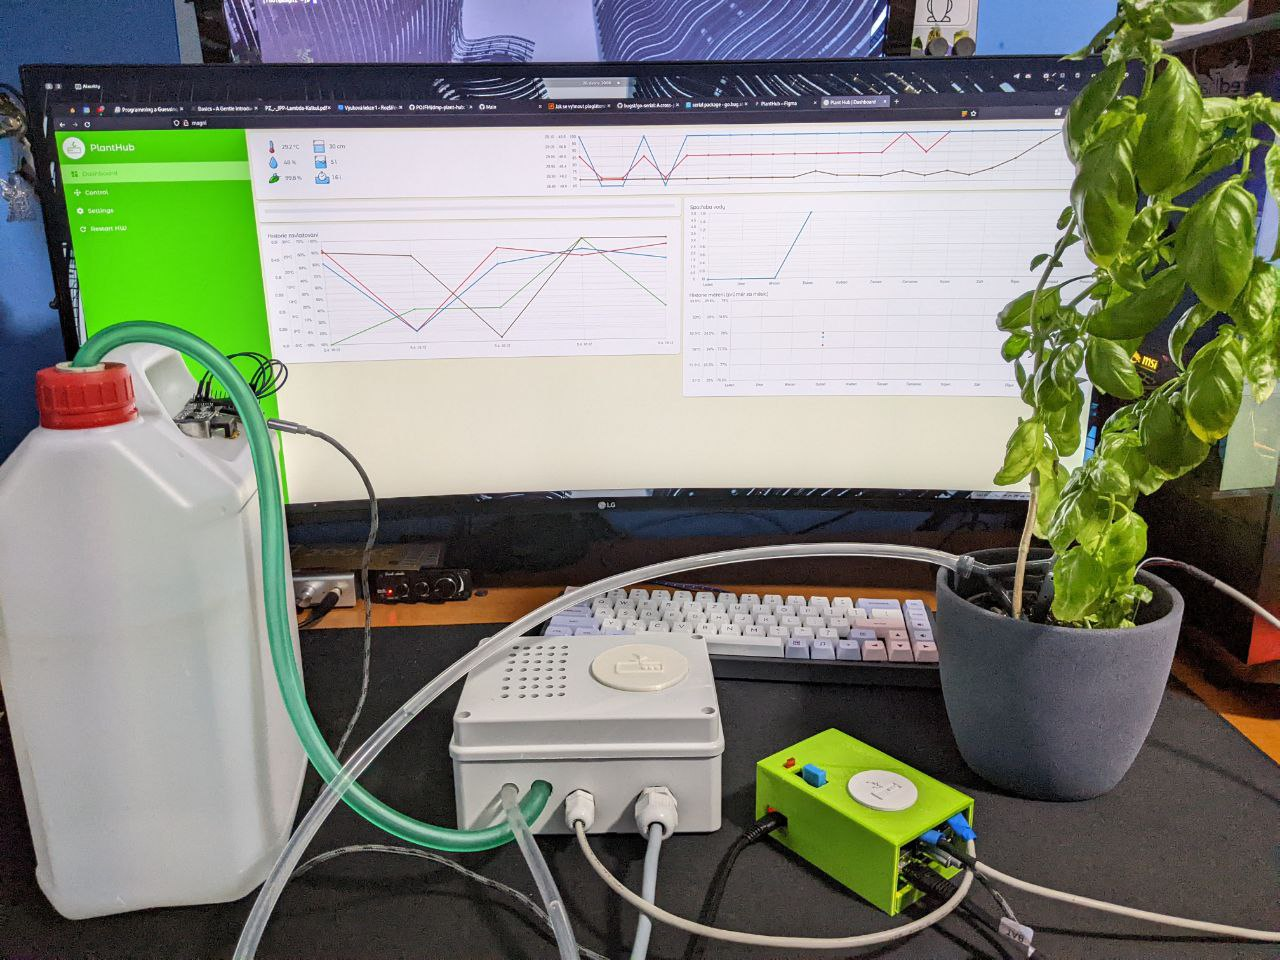
\includegraphics[width=0.9\linewidth]{planthub.jpeg}
	\caption{Celý systém}
\end{figure}

\clearpage

\section{Hlavní program} \label{secProgram}

\subsection{Postup práce}

Náš hlavní program pro zavlažování, komunikaci s databází a \underline{\ac{WUI}} jsme začali psát ve vysokoúrovňovém programovacím jazyce Python. Od toho jsme nakonec upustili, kvůli horšímu výkonu. Program jsme přepsali v programovacím jazyku Go.

\begin{figure}[h]
	\centering
	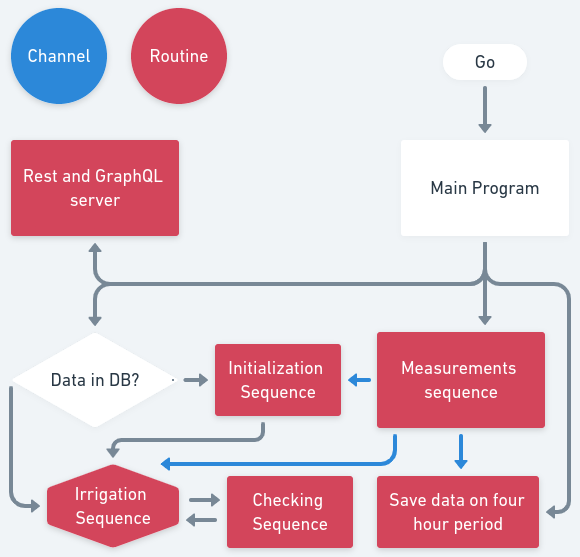
\includegraphics[width=0.72\linewidth]{go.png}
	\caption{Vývojový diagram programu}
\end{figure}

\subsection{Fáze programu}

Fáze programu se spouštějí buďto v samostatné go rutině a komunikují spolu pomocí kanálů, nebo na základě podmínek, kde se po splnění požadavků ukončí.

\subsubsection{Měření}

Senzor vlhkosti půdy a \underline{\ac{DHT11}} průběžně posílají naměřená data do \underline{\ac{WUI}}. Hlavní program ve stejné chvíli čte data ze senzorů a kontroluje jestli naměřené hodnoty nepřekračují limitní hodnoty vlhkosti půdy pro spuštění zavlažování, a ve stejné chvíli kontroluje jestli jestli není čas spustit čerpadlo podle plánovaného zavlažování. Pokud ano, \underline{\ac{RPi}} pošle signál pro otevření tranzistoru, což spustí čerpadlo.

\subsubsection{Periodické ukládání dat}

V samostatné rutině běží funkce pro ukládání naměřených dat v periodě 4 hodin. Tato rutina, stejně jako ostatní, čte hodnoty senzorů z měřící sekvence. Naměřená data jsou následně statisticky zobrazena ve \underline{\ac{WUI}}.

\subsubsection{Controller}

Po spuštění měřící sekvence a sekvence periodického ukládání dat, se spustí buďto inicializační sekvence, nebo zavlažovací sekvence. Podle toho, jestli se v databázi nachází předchozí nastavení. Pokud předchozí nastavení nejsou nalezena, program čeká na uložení dat z \space \underline{\ac{WUI}} a \ac{LED} bliká dvakrát po sobě, dokud data nejsou dostupná. Pokud jsou data k dispozici, spustí se zavlažovací sekvence a načtou se limitní data z databáze. V periodě jedné sekundy se budou číst data o vlhkosti půdy.

\subsubsection{Inicializace}

Půda musí být ze začátku suchá. Senzor vlhkosti půdy zasuneme co nejhlouběji do půdy. \underline{\ac{RPi}} bude chvíli sbírat data a pak je zprůměruje do hodnoty, která bude sloužit jako limit pro spuštění čerpadla.

Ve \underline{\ac{WUI}} jde navíc ještě manuálně nastavit hranice vlhkosti půdy pro spuštění čerpadla.

Nastavit se dá také množství vody, které bude přečerpáno při jednom spuštění a jaká je hranice pro přijatelnou výšku hladiny vody v nádrži. Pokud nejsou tyto hodnoty uvedeny, čerpadlo bude vodu přečerpávat, dokud se nezmění hodnota kapacitního čidla pro měření vlhkosti půdy a \space \underline{\ac{HC-SR04}} použije výchozí nastavení.

\subsubsection{Zavlažování}

Čerpadlo začne čerpat vodu a zavlažovat rostlinu. Voda se čerpá tak dlouho, dokud senzor vlhkosti půdy nezmění svou hodnotu, nebo dokud není vyčerpán limit přečerpané vody na jedno spuštění.

\subsubsection{Kontrola}

Po ukončení přečerpávání se spustí \underline{\ac{HC-SR04}} a změří výšku hladiny vody. Naměřená data poté odešle do \underline{\ac{RPi}}, kde se uloží do databáze. Pokud bude naměřená hodnota nižší, než je limitní hodnota, začne blikat \underline{\ac{LED}} a \underline{\ac{RPi}} odešle upozornění o doplnění nádrže do \underline{\ac{WUI}}. Jakmile bude hladina vody doplněna, signalizace se vypne.

\subsubsection{Ukládání dat}

Náš systém ukládá zvlášť periodicky naměřená data a data naměřená před zavlažováním. Dále ukládá nastavení jak pro limity k zavlažování, tak pro \underline{\ac{WUI}}.

\subsection{Programovací jazyk Go}

Go je open-source programovací jazyk, který byl vytvořen společností Google v roce 2009. Je to stále relativně nový programovací jazyk, který se nevyvinul z jiných jazyků jako C\# a Java. Go ignoruje teorii o programovacích jazycích. Místo toho, aby se zaměřoval na akademické teorie, zaměřuje se na reálné praktiky, používané pro vývoj next-gen v cloudových, distribuovaných a souběžných aplikacích.

Jazyk Go je staticky typovaný a využívá garbage collector (automatický správce paměti). Jedná se o kompilovaný programovací jazyk, který své binární soubory kompiluje pro každou platformu. Dá se zařadit do skupiny C jazyků, podle jeho základní syntaxe. Go poskytuje expresivní syntax s jednoduchým typovým systémem a má vestavěné nástroje pro paralelní programování. Výkon Go je srovnatelný s jazyky C a C++, ale zároveň nabízí rychlý a jednoduchý vývoj aplikací.

Stejně jako C a C++ se Go kompiluje do nativního strojového kódu, takže
nepotřebujeme běhové prostředí jako Common Language Runtime (CLR) a Java Virtual Machine (JVM). To má řadu výhod, třeba při distribuci aplikace v aplikačních kontejnerech, jako je Docker.

\subsubsection{Paralelní programování v Go}

Vývoj počítačů se v průběhu posledního desetiletí značně posunul. V minulosti aplikace běžely na počítačích pouze s jediným procesorovým jádrem. Dnes jsou standartně k vidění čtyřjádrové procesory v uživatelských počítačích, dokonce i naše \underline{\ac{RPi}} má dvě jádra. Stále používáme programovací jazyky a technologie navržené v éře, kdy byly dostupné pouze jednojádrové procesory.

Většina programovacích jazyků dnes nabízí knihovny, nebo frameworky pro \linebreak paralelní programování, ale nemají tuto vlastnost zabudovanou přímo v jádře jazyka. V Go je paralelní programování součástí jazyka už od samotného počátku. Používá takzvané Gorutiny, které umožňují spouštět funkce souběžně. Souběžné funkce pak mezi sebou mohou komunikovat a předávat data pomocí kanálů. Dokonce i některé standardní knihovny jazyka mají zabudovanou souběžnost. Například standardní knihovna `net/http' pro programování HTTP, zpracovává přicházející požadavky souběžně pomocí Gorutin.

\subsubsection{Typový systém}

Pragmatický design Go neobsahuje klíčové slovo pro třídu a jeho objektová orientace je odlišná od tradičních, objektově orientovaných programovacích jazyků. V Go nahrazuje funkci tradiční třídy typ struct. Dědění není v go podporováno, ale podporuje kompozici typů (Příloha 1).

\clearpage

\section{WUI} \label{secWUI}

\subsection{Programování WUI}

Webovovou aplikaci jsme napsali pomocí javascriptového frameworku
React.js, CSS frameworku Tailwind a programovacího jazyku Typescript, který je dialektem javascriptu, podporující volitelné statické typování. JavaScript je dynamicky typovaný jazyk. Statické typování je výhodné hlavně u větších aplikací, kde zjednodušuje odchytávání chyb v oblasti datových typů, nebo jim předchází úplně.

Ve webovém rozhraní je možné zobrazit si statisky, jak živě naměřených dat, tak dat uložených v databázi. Z OpenWeather \underline{\ac{API}} získáváme data o předpovědi počasí a do dahsboardu zobrazujeme předpovědi na dalších 15h.

\subsection{Inicializační formulář}

\begin{figure}[h]
	\centering
	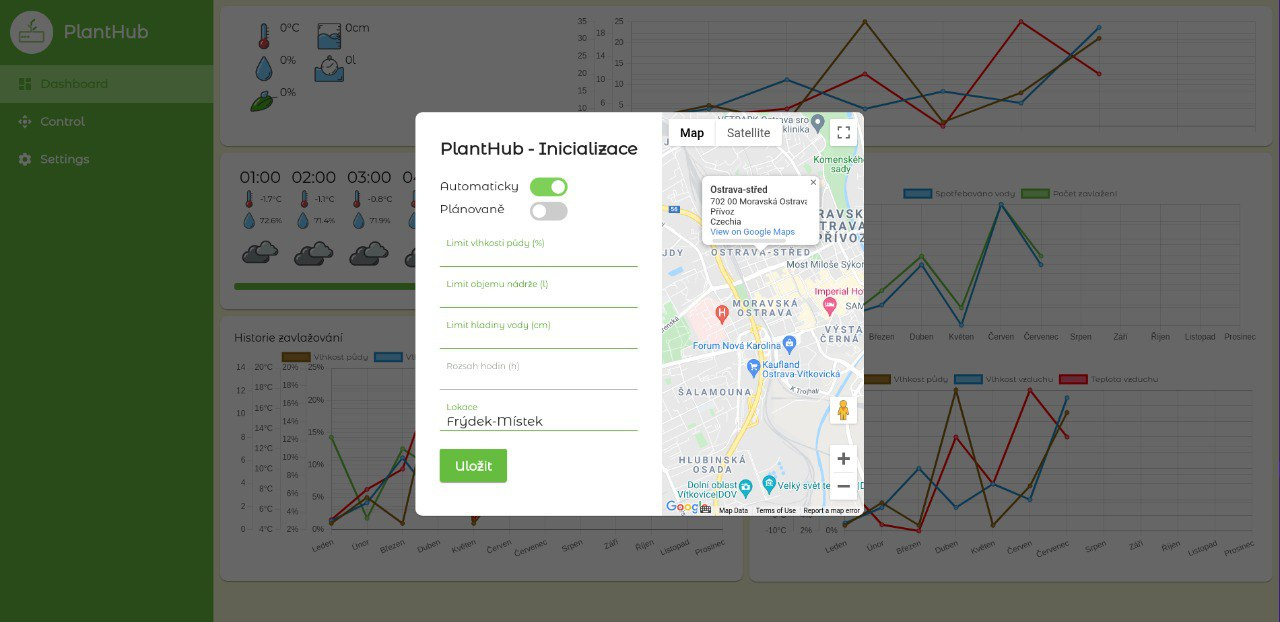
\includegraphics[width=\linewidth]{ui-inicializace.jpg}
	\caption{Inicializační formulář}
\end{figure}

Okno prvotního nastavení obsahuje uživatelsky přívětivé rozhraní, které uživatele provede nastavením systému. Nastaví se mód zavlažování, limitní hodnoty a lokace, ze které má PlantHub ukazovat předpověď počasí.

\clearpage

\subsection{Dashboard}

\begin{figure}[h]
	\centering
	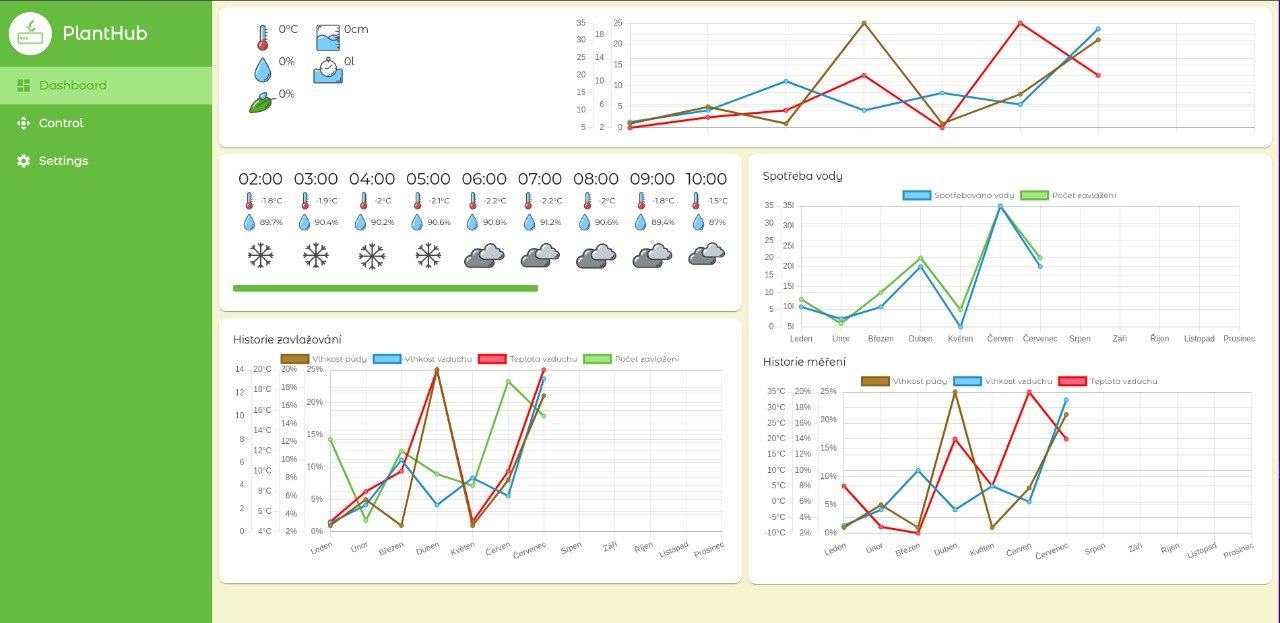
\includegraphics[width=\linewidth]{web-ui.png}
	\caption{Dashboard}
\end{figure}

Prostředí dashboardu (nástěnky) je hlavní částí webové aplikace. Uživatel zde může sledovat aktuální dění v podobně real-time dat ze senzorů a aktuálního stavu nádrže. K tomu jsme mu připravili praktickou kartu s předpovědí počasí a karty s grafy historických dat.

Prvním takovýmto grafem je historie zavlažování. Tento graf zobrazuje statisticky jaká byla teplota, vlhkost vzduchu a vlhkost půdy, těsně před zavlažováním. Na pravé straně jsou umístěny další dva grafy, první zobrazuje spotřebu vody při zavlažování za jednotlivé měsíce. Druhý potom vykresluje historické průměry naměřených dat v jednotlivých měsících.

\clearpage

\subsection{Manuální ovládání}

\begin{figure}[h]
	\centering
	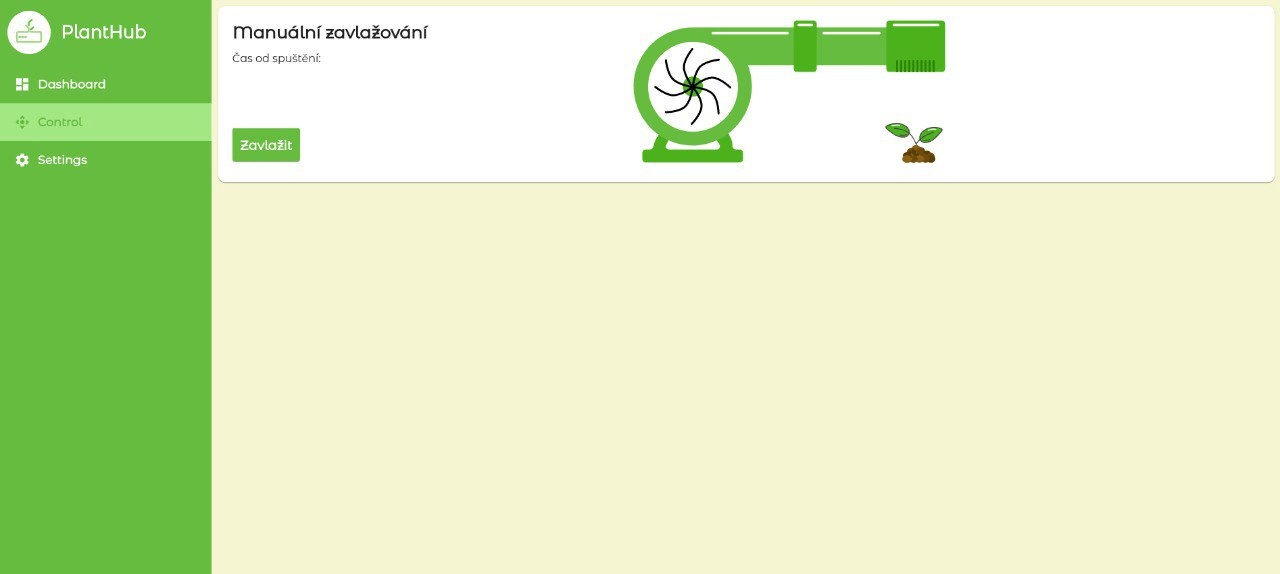
\includegraphics[width=\linewidth]{web-ui-pump.png}
	\caption{Manuální ovládání}
\end{figure}

Manuální ovládání čerpadla dovoluje uživateli kdykoliv spustit zavlažování. Po dokončení manuálního zavlažování, se také spustí kontrola hladiny vody v nádrži. Při úpravě limitních hodnot, či jiných nastavení řídící jednotky, je nutno zařízení restartovat. K tomu v menu \underline{\ac{WUI}} slouží možnost \enquote{Restart HW}.

\clearpage

\subsection{Nastavení}

\begin{figure}[h]
	\centering
	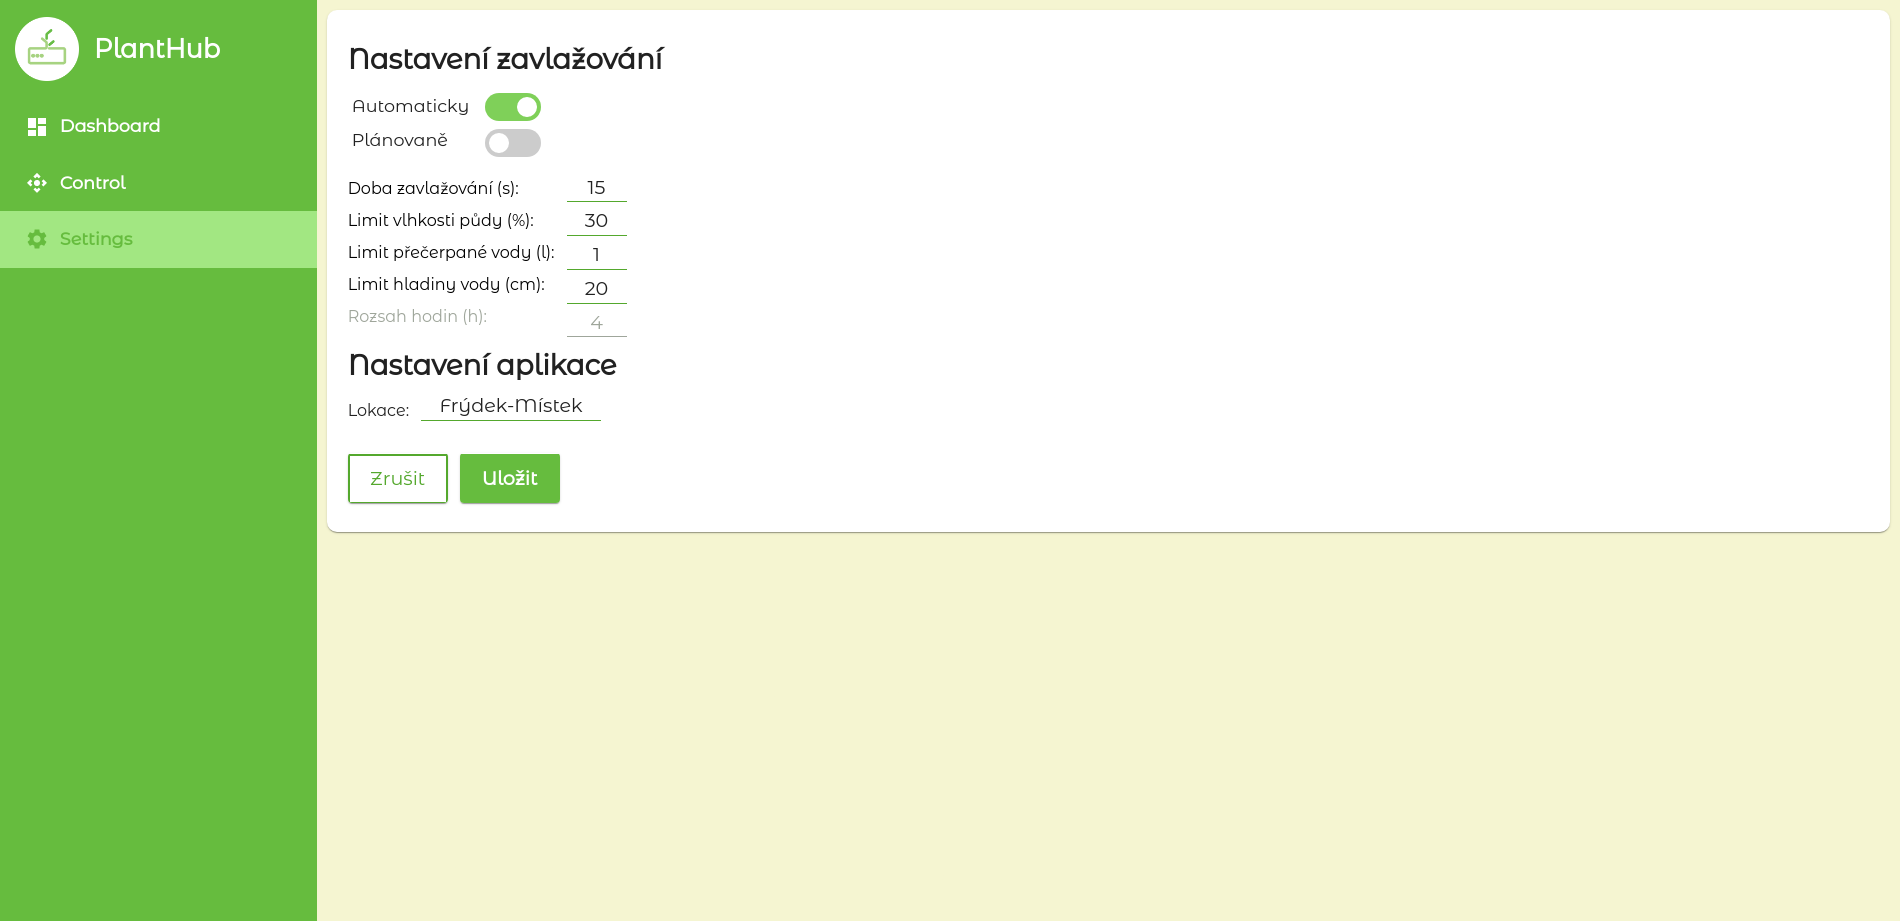
\includegraphics[width=\linewidth]{web-ui-settings.png}
	\caption{Nastavení}
\end{figure}

V nastavení lze změnit nastavení aplikace, včetně limitů pro zavlažování a doby zavlažování. Na výběr máme automatické a plánované zavlažování. V prvním režimu PlantHub zavlažuje automaticky, kdy a jak moc má zavlažit, vyhodnotí z dat senzoru vlhkosti půdy. Při plánovaném zavlažování nastavíme intervaly, ve kterých se má zavlažovat. V nastavení aplikace se nastavuje lokace pro předpověď počasí. Nastavení se ukládají do databáze.

\clearpage

\subsection{Notifikace}

\begin{figure}[h]
	\centering
	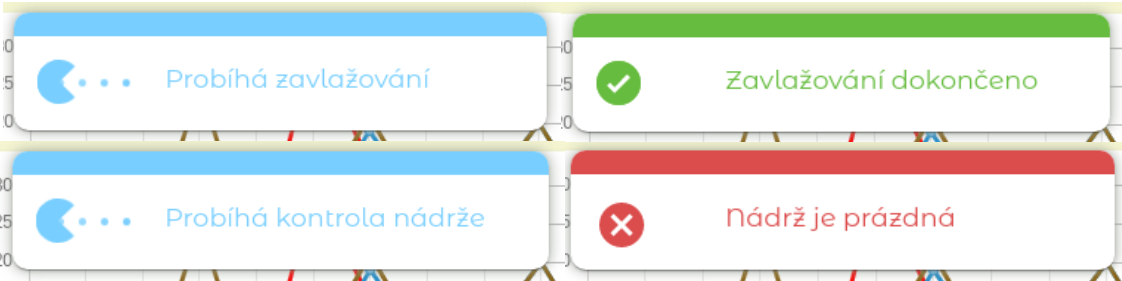
\includegraphics[width=\linewidth]{notifikace.png}
	\caption{Sada notifikací}
\end{figure}

Součástí webového rozhraní jsou i praktické notifikace, které uživatele upozorňují na aktuální stav PlantHubu. Poskytují vizuální zpětnou vazbu, při průběhu zavlažování a kontrole nádrže. Při úspěšném dokončení zavlažování, informují uživatele. V případě, že je nádrž na vodu prázdná, tak uživatele s touto skutečností seznámí.

\clearpage

\section{Databáze} \label{secDB}

\subsection{SQL}

Pro databázi jsme se rozhodli použít databázový systém PostgreSQL.\@ Jak vyplývá z názvu, jedná se o Structured Query Language (SQL) databázi, ty jsou vhodné pro ukládání velkého objemu dat, jako právě data z našich senzorů. Webová aplikace používá pro přístup k datům z databáze \ac{GraphQL} \space \underline{\ac{API}}.\@

\subsection{GraphQL} \label{secGraphQL}

Jedná se o typ přenosu dat z možností filtrace a dotazovací funkcionality. V mnoha ohledech je to konkurent řešení přenosu dat pomocí \ac{REST} \space \underline{\ac{API}}.\@ Nabízí rychlejší tvorbu \underline{\ac{API}} \space a také umožňuje efektivnější přístup k datům z databáze. Umožňuje vybrat pouze data, která momentálně aplikace používá a dovoluje vynechat data, která zrovna potřebná nejsou.

\subsection{Schéma databáze}

\begin{figure}[h]
	\centering
	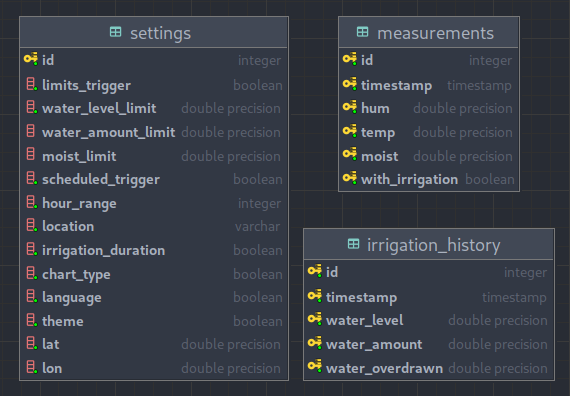
\includegraphics[width=0.8\linewidth]{db.png}
	\caption{Schéma databáze}
\end{figure}

\clearpage

\section{Webový server} \label{secWebServer}

Web server jsme napsali v moderním jazyku Go, který nyní získává na popularitě, hlavně mezi cloudovými vývojáři a v oblasti vývoje microservices. Dokáže se v rychlosti provedení programu přiblížit k nízkoúrovňovým jazykům, jako je C nebo Rust, ale zároveň zůstává velmi lidsky čitelný a jednoduchý na použití. Na rozdíl od jazyků jako C a Rust, má například garbage collector (automatický správce paměti), který periodicky čistí paměť a zabraňuje memory leakům.

\clearpage

\section{Docker a kontejnerizace} \label{secDocker}

% Docker kontejner si můžeme představit jako takový odlehčený virtuální počítač, ale s lepší škálovatelností a cílením hlavně na prostředí, důležité pro vývoj aplikací. Jde především o izolaci \underline{\ac{WUI}} od hostovaného systému, a plnou kontrolu nad prostředím \underline{\ac{WUI}}, databáze a hlavního programu.

Kontejnerizace je zabalení aplikace spolu se všemi nutnými komponenty, jako jsou knihovny, frameworky a další závislosti (dependencies), do svého vlastního \enquote{kontejneru}, který je izolovaný od zbytku systému.

Daná aplikace nebo program, potom může být spuštěna konzistentně kdekoliv, nezávisle na prostředí, operačním systému i architektury hostového systému. Aplikace běží zcela nezávisle na zbytku systému. Kontejner imituje jakousi bublinu, která aplikaci obklopuje a izoluje. Je to v podstatě plně funkční a přenosné výpočetní prostředí. Toto je hlavním důvodem, proč jsme zvolili kontejnerizaci pro náš projekt. V případě, že bychom chtěli vyrobit více jednotek, tak můžeme na jednotlivé Raspberry Pi nasadit předpřipravené kontejnery a nemusíme se skoro vůbec zabývat konfigurací operačního systému Raspberry Pi.

Kontejnery poskytují alternativu ke klasickému vývoji aplikací na jedné platformě, nebo operačním systému. Tento přístup může zhoršit kompatibilitu aplikace s jinými systémy, které nemusí sdílet stejné prostředí, jako systém, na kterém byla aplikace původně vyvíjena. Tato zhoršená kompatibilita může způsobit všelijaké problémy a chyby aplikace, které se potom musí řešit navíc. V realitě to pak znamená prodloužený čas vývoje, snížení produktivity a frustraci vývojářů.

Díky zabalení aplikace v kontejneru, pak může být jednoduše spouštěna napříč platformami a operačními systémy. Také ji můžeme jednoduše přesouvat mezi zařízeními, protože vše co potřebuje, má zabaleno ve svém kontejneru.

Myšlenka kontejnerizace existuje dlouho. Docker, ale v roce 2013 stanovil standart kontejnerizace technologií Docker Engine. Docker Engine přinesl jednoduché nástroje pro vývoj, díky nimž se stal vývoj s použitím kontejnerů snadný. Zavedl také univerzální přístup k distribuci kontejnerů, což zrychlilo adopci kontejnerizace. Dnes si vývojáři mohou vybrat z nabídky kontejnerizačních platforem, které podporují standart Open Container Initiative, vyvinuté společností Docker.

\subsection{Výhody kontejnerizace}

Kontejnery sdílejí kernel (jádro) operačního systému s jejich hostem. Kontejnery tak nepotřebují svůj vlastní operační systém a díky tomu jsou výpočetně nenáročné. Můžou tak běžet stejně na jakémkoliv zařízení, ať už se jedná o malé Raspberry Pi, nebo cloudové datacentra.

\subsection{Kontejnery vs. virtuální počítače}

Virtuální počítač je virtuální prostředí, které funguje jako běžný počítač. Má svůj vlastní virtuální procesor, paměť, síťový adaptér a úložiště. Tyto komponenty jsou virtualizovány na fyzickém hardwaru hostujicího systému.

Kontejnerizace a virtualizace jsou podobné v tom, že poskytují plnou izolaci aplikace, aby byla jednoduše spustitelná v různých typech prostředí. Hlavním rozdílem je velikost, výpočetní náročnost a přenosnost.

Virtuální počítač je větší z této dvojice, jeho velikost je typicky měřena v gigabytech. Obsahuje svůj vlastní operační systém, který mu dovoluje provádět několik výpočetně náročných funkcí zároveň. Jeho zvýšený výpočetní výkon, mu umožňuje zapouzdřit, rozdělit, duplikovat a emulovat celé servery, operační systémy, desktopy, databáze a počítačové sítě.

Kontejnery jsou mnohem menší, velikostí většinou v řádech megabytů a neobsahují nic víc, než samotnou aplikaci a nutné prostředí pro její běh.

Virtuální počítače fungují dobře v tradičních a monolitických IT architekturách. Kontejnery byly navrženy s důrazem na nejnovější a vznikající technologie, jako cloudy, CI/CD a DevOps.

\clearpage

\section{Bezpečnost} \label{secBezpecnost}

Náš projekt spadá do kategorie zařízení IoT, neboli Internet of Things. Česky by to byl \enquote{Internet věcí}. Bezpečnost IoT zařízení bylo vždy velké téma. Zařízení IoT jsou totiž nechvalně známé svou nedostatečnou bezpečností. Tyto zařízení často bývají pro útočníky pomyslnou bránou do lokální sítě jejich oběti.

Rozmach těchto zařízení u běžných lidí tento problém zvýraznil. Mezi poslední trendy technologie patří chytré domy, kde je vše ovládáno chytrými zařízeními, které lze nastavovat na dálku pomocí telefonu. Hlavní charakteristikou IoT je schopnost zařízení připojit se k internetu, a interagovat se svým okolím pomocí sběru a výměny dat. Jedná se o zařízení od chytrých ledniček, termostatů, automatických vysavačů a žaluzií až po žárovky. Tím že jsou všechny tyto zařízení připojeny k internetu, jen zvyšujeme šanci napadení.

Náš projekt je zcela nezávislý na serverech v cloudu, místo toho je komunikace s PlantHubem zprostředkována pouze v lokální síti. Tímto designem jsme sice znemožnili přístup k PlantHubu mimo lokální síť, ale zároveň jsme velmi pozitivně ovlivnili bezpečnost celého systému. Zařízení stále musí být připojeno k internetu, z důvodu získávání dat ohledně předpovědi počasí a polohy z \underline{\ac{API}} třetí strany. K přístupu a možnosti ovládání mimo lokální síť bychom potřebovali VPN server v lokální síti.

K tomu jsme vybrali Fedora IoT jako naši linuxovou distribuci. Tato distribuce je přímo určená zařízením jako je naše, jak již vyplývá z názvu distribuce. Byla navržena s velkým důrazem na bezpečnost a základní nastavení distribuce je velmi bezpečné. Mezi bezpečnostní funkce patří SecureBoot, automatické šifrování úložiště, firewall a další.

\clearpage

\section{Závěr} \label{secZaver}

Náš projekt je stále ve vývoji a některé z funkcí tohoto projektu, nefungují podle našich představ. I přes to, je náš systém v této chvíli použitelný. Myslíme si, že tento projekt má v budoucnu potenciál stát se úspěšným startupem. Proto plánujeme pokračovat v jeho vývoji i po maturitě.

Abychom však tento projekt mohli pojmout jako plně funkční systém, museli bychom ještě dokončit a předělat některé klíčové části. Jednalo by se především o rozdělení hostingu webové aplikace a databáze na samostatný server. Zajištění modulárnosti celého systému rozdělením řídící jednotky na samostatné moduly a hub zodpovědný za jejich provoz. V dalších neprioritních krocích, se můžeme bavit o dokončení plánované tmavé verze \underline{\ac{WUI}} a přidání podpory více jazyků. Pro odlišení od konkurence mnoha jiných zavlažovacích systémů, přidáme chytré funkce vypočítávání spotřeby vody, energie a na základě předpovědi počasí, typu rostliny a lokace. Uvažovali jsme také nad soukromou databází rostlin a jejich rozdělení, na základě způsobu pěstování. V komerčním modelu, bychom mohli z této databáze vytvořit placené \underline{\ac{API}}, pro jiné zavlažovací systémy.

Tato práce, byla pro nás velkým přínosem. Naučili jsme se mnoho nových dovedností a načerpali nové informace, které v naší profesi bezpochyby dále využijeme.

\clearpage

\section{Seznam obrázků} \label{secObrazky}

\vspace*{-1.5cm}
\listoffigures

\clearpage

\section{Reference} \label{secReference}

\begin{thebibliography}{9}
	\vspace*{-1.5cm}
	\bibitem{texbook}
	“Home,” LaTeX, 06-May-2021. [Online]. Dostupné z: \underline{\href{https://latex-tutorial.com/}{https://latex-tutorial.com/}}. [Zpřístupněno: 10-Dubna-2022]. 

	\bibitem{golang}
	“Build fast, reliable, and efficient software at scale,” Go. [Online]. Dostupné z: \underline{\href{https://go.dev/}{https://go.dev/}}. [Zpřístupněno: 10-Dubna-2022]. 

	\bibitem{react}
	“React – a JavaScript library for building user interfaces,” – A JavaScript library for building user interfaces. [Online]. Dostupné z: \underline{\href{https://reactjs.org/}{https://reactjs.org/}}. [Zpřístupněno: 10-Dubna-2022]. 

	\bibitem{tailwindcss}
	“Rapidly build modern websites without ever leaving your HTML.,” Tailwind CSS. [Online]. Dostupné z: \underline{\href{http://www.tailwindcss.com/}{http://www.tailwindcss.com/}}. [Zpřístupněno: 10-Dubna-2022]. 

	\bibitem{typescript}
	“JavaScript with syntax for types.,” TypeScript. [Online]. Dostupné z: \underline{\href{http://www.typescriptlang.org/}{http://www.typescriptlang.org/}}. [Zpřístupněno: 10-Dubna-2022]. 

	\bibitem{vscode}
	Microsoft, “Visual studio code - code editing. redefined,” RSS, 03-Nov-2021. [Online]. Dostupné z: \underline{\href{https://code.visualstudio.com/}{https://code.visualstudio.com/}}. [Zpřístupněno: 10-Dubna-2022]. 

	\bibitem{goland}
	“Goland by jetbrains: More than just A go ide,” JetBrains. [Online]. Dostupné z: \underline{\href{https://www.jetbrains.com/go/}{https://www.jetbrains.com/go/}}. [Zpřístupněno: 10-Dubna-2022]. 

	\bibitem{git}
	Git. [Online]. Dostupné z: \underline{\href{https://git-scm.com/}{https://git-scm.com/}}. [Zpřístupněno: 10-Dubna-2022]. 

	\bibitem{figma}
	“The Collaborative Interface Design Tool.,” Figma. [Online]. Dostupné z: \underline{\href{https://www.figma.com/}{https://www.figma.com/}}. [Zpřístupněno: 10-Dubna-2022]. 

	\bibitem{freecad}
	“Freecad,” FreeCAD. [Online]. Dostupné z: \underline{\href{https://www.freecadweb.org/}{https://www.freecadweb.org/}}. [Zpřístupněno: 10-Dubna-2022]. 

	\bibitem{easyeda}
	An easier and PowerfulOnline PCB design tool. EasyEDA. [Online]. Dostupné z: \underline{\href{https://easyeda.com/}{https://easyeda.com/}}. [Zpřístupněno: 10-Dubna-2022]. 
\end{thebibliography}

\clearpage

\section{Seznam použitého softwaru} \label{secSoftware}

\begin{enumerate}
	\item Visual Studio Code
	\item GoLand
	\item EasyEDA
	\item FreeCAD
	\item Figma
	\item Git
\end{enumerate}

\clearpage

\section{Seznam příloh} \label{secSeznamPriloh}

\begin{itemize}
	\item Příloha 1: Typový systém v Go.png
	\item Příloha 2: Zdrojový kód
	\item Příloha 3: Modely krytu
	\item Příloha 4: Prezentace.pdf
\end{itemize}

\clearpage

\section{Přílohy} \label{secPrilohy}

\end{document} 